

%\subsection{Alternative to DGLAP DIS models}
Different approaches that are alternative to the DGLAP formalism can be used to analyse DIS data in \fitter.
These include several different dipole models and the use of 
transverse momentum dependent, or unintegrated PDFs, uPDFs.
These approaches are discussed below.

\subsection{DIPOLE models}

The dipole picture provides an alternative approach to virtual photon-proton
 scattering at low $x$ which allows the description of both inclusive and 
diffractive processes.
 In this approach, the virtual photon fluctuates into a $q\bar q$ (or $q\bar q g$) 
 dipole which interacts with the proton~\cite{NNZ:91}.  
The dipoles can be viewed as quasi-stable quantum mechanical states, which have very long 
life time $\propto 1/m_p x\;$ and a size which is not changed by scattering.
%A schematic view of dipole factorisation at small $x$ in DIS is illustrated in figure~\ref{fig:dipole}.
The dynamics of the interaction are embedded in the dipole scattering amplitude.

%\begin{figure}
%\begin{center}
%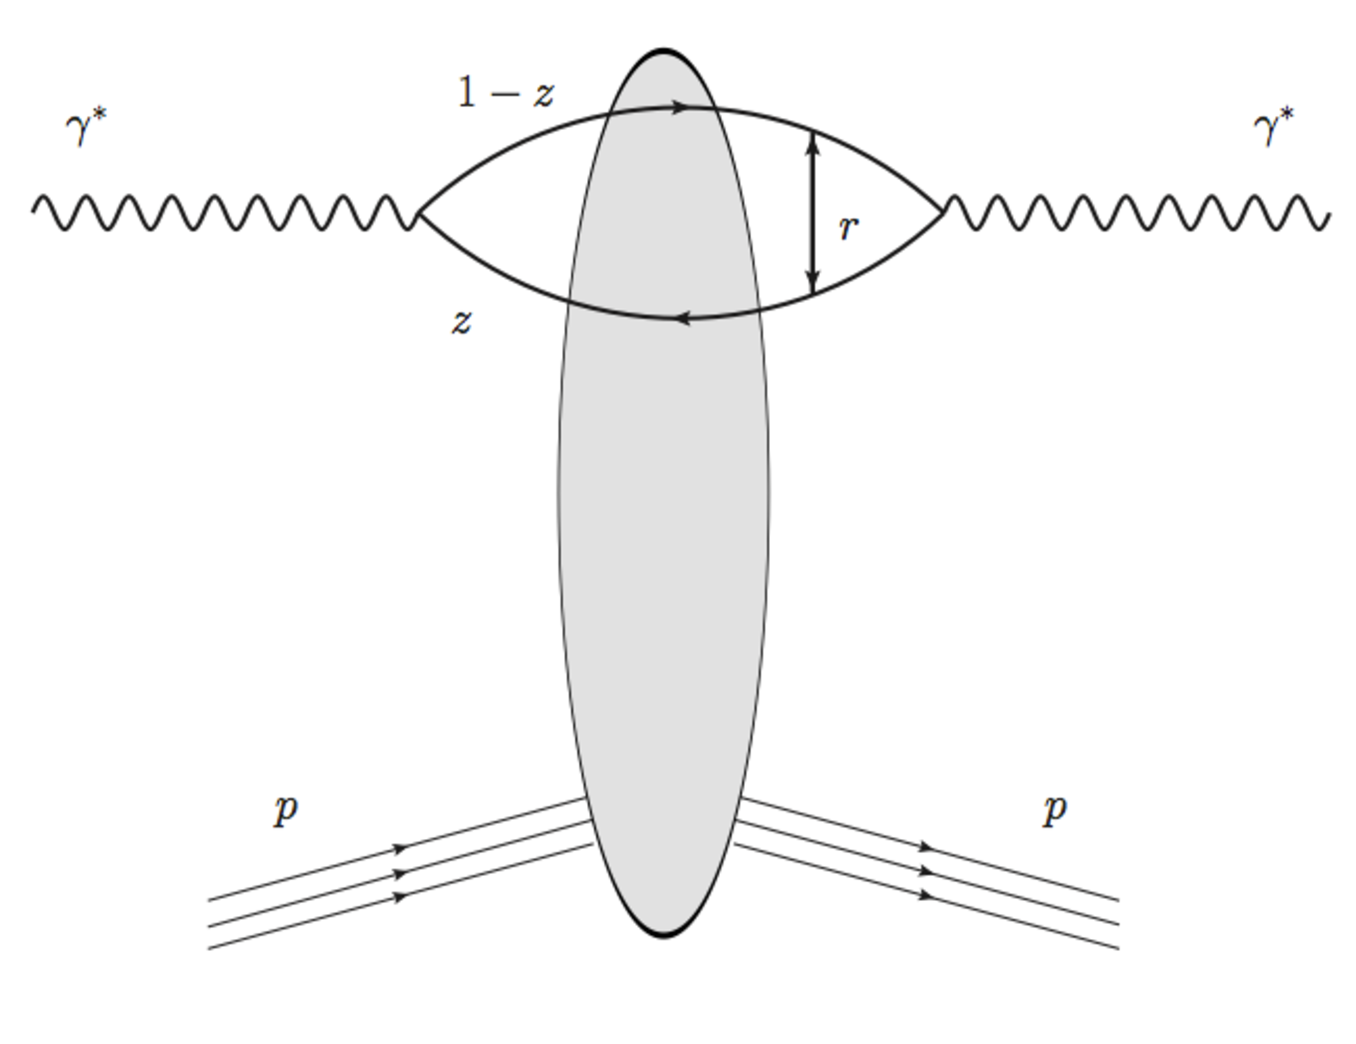
\includegraphics[width=0.5\linewidth]{figures/dipole.pdf}
%\end{center}
%\caption{Schematic diagram of dipole factorisation for the inclusive cross section in DIS.}
%\label{fig:dipole}
%\end{figure}

Several dipole models which assume different behavior of the dipole-proton 
cross sections are implemented in \fitter:
%\begin{itemize}
%\item the original Golec-Biernat-W\"usthoff (GBW)~\cite{Golec-Biernat:1998js} 
the Golec-Biernat-W\"usthoff (GBW)
dipole saturation model~\cite{Golec-Biernat:1998js},
the colour glass condensate approach to the high parton density 
regime called the Iancu-Itakura-Munier (IIM) dipole model~\cite{Iancu:2003ge} and 
a modified GBW model which takes into account the effects of  
DGLAP evolution called the Bartels-Golec-Kowalski (BGK) dipole model~\cite{Bartels:2002cj}.
%\end{itemize}

\begin{description}
\item \bf {GBW model:} \rm
In the GBW model the dipole-proton cross section $\sigma_{\text{dip}}$ is given by
\begin{equation}
\label{eGBW}
   \sigma_{\text{dip}}(x,r^{2}) = \sigma_{0} \left(1 - \exp \left[-\frac{r^{2}}{4R_{0}^{2}(x)} \right]\right),
\end{equation}
here $r$ corresponds to the transverse separation between the quark and the antiquark, and $R_{0}^{2}$
 is 
%an $x$ dependent scale parameter, having the form $R_{0}^{2}(x)=\left(x/x_{0}\right)^{\lambda}$.
an $x$-dependent scale parameter which represents the spacing of the gluons in the proton. $R_{0}^{2}(x)=\left(x/x_{0}\right)^{\lambda}$ is called the saturation radius.
The fitted parameters are the cross-section normalisation $\sigma_{0}$ and $x_{0}$ and $\lambda$. This model gives exact Bjorken scaling when the dipole size $r$ is small.
%%%%

\vspace{0.1cm}
\item \bf {IIM model:} \rm
The IIM model assumes an improved expression for the dipole cross section which is based on the 
Balitsky-Kovchegov equation~\cite{Balitsky:1995ub}. The explicit formula for $\sigma_{\text{dip}}$ 
can be found in~\cite{Iancu:2003ge}. The fitted parameters are an alternative scale parameter $\tilde{R}$, $x_{0}$ and $\lambda$.
%%%%

\vspace{0.1cm}
\item \bf {BGK model:} \rm
The BGK model modifies the GBW model by taking into account the  DGLAP evolution
of the gluon density. 
The dipole cross section is given by
\begin{equation}
\begin{array}{lcl}
   \sigma_{\text{dip}}(x,r^{2})  =  \sigma_{0} 
\left(1 - \exp \left[-\frac{\pi^{2} r^{2} \alpha_{s}(\mu^{2}) xg(x,\mu^{2})}{3 \sigma_{0}} \right]\right).
\end{array}
\label{eBGK}
\end{equation}
The factorization scale $\mu^{2}$ has the form $\mu^{2} = C_{bgk}/r^{2}+\mu^{2}_{0}$.
%This model uses the following gluon density at the starting scale $Q_{0}^{2}=1\mbox{ GeV}^{2}$.
This model relates to the GBW model using the idea that the spacing $R_0$ is inverse to the gluon density.
The gluon density parametrized at some starting scale $Q_{0}^{2}$ by
$ xg(x) = A_{g} x^{-\lambda_{g}}(1-x)^{C_{g}} $
is evolved to larger scales using LO or NLO DGLAP evolution.
The fitted parameters for this model are $\sigma_{0}$, $\mu^{2}_{0}$ and three parameters for the gluon density: $A_{g}$, $\lambda_{g}$, $C_{g}$. The parameter $C_{bgk}$ is kept fixed: $C_{bgk} = 4.0$. 
%%%%

\vspace{0.1cm}
\item \bf {BGK model with valence quarks:} \rm

The dipole models are valid in the low-$x$ region only, where the valence quark contribution is small, of the order of 5\%. The new HERA $F_2$ data have a precision which is  better than 2 \%. Therefore, in \fitter\ the contribution of the valence quarks is taken from the PDF fits and added to the original 
BGK model, this is uniquely possible within the \fitter\ framework.
% The quality of the fits of the BGK dipole model with valence quarks and without 
%valence quarks are the same.
\end{description}

\subsection{Transverse Momentum Dependent  PDFs with CCFM}

Here another alternative approach to collinear DGLAP evolution is presented.
In high energy factorization \cite{Catani:1990eg} the measured cross section is written
 as a convolution of the partonic cross section $\hat{\sigma}(É \kt),$ which depends on the transverse 
momentum $\kt$ of the incoming parton, with the $\kt$-dependent parton distribution function 
${\cal \tilde A}\left(x,\kt,\Pmax\right)$ (transverse momentum dependent (TMD) or unintegrated uPDF):
\begin{equation}
 \sigma  = \int 
\frac{dz}{z} d^2k_t \hat{\sigma}(\frac{x}{z},k_t)  {\cal \tilde A}\left(x,\kt,\Pmax\right)
\label{kt-factorisation}
\end{equation}
%{\bf would probably be good to explain how the unintegrated relates to the integrated here}
Generally, the evolution of ${\cal \tilde A}\left(x,\kt,\Pmax\right)$ 
can proceed via the BFKL\cite{BFKL}
%{\bf you need a BFKL reference},
 DGLAP or via the CCFM evolution equations.
In \fitter, an extension of the CCFM~\cite{\CCFM} evolution has been implemented.
Since the evolution cannot be easily obtained in  a closed form, 
 first a kernel $ {\cal \tilde A}\left(x'',\kt,\Pmax\right) $ 
is determined from the MC solution of the CCFM evolution equation, 
and is then folded with a non-perturbative starting distribution 
${\cal A}_0 (x)$~\cite{Jung:2012hy}:
\begin{eqnarray}
%\begin{align}
 x {\cal A}(x,\kt,\Pmax) & = & 
   x\int dx' \int dx'' {\cal A}_0 (x) {\cal \tilde A}\left(x'',\kt,\Pmax\right)  \delta(x' \cdot x'' - x) \nonumber \\  
 & = & \int dx' \int dx'' {\cal A}_0 (x) {\cal \tilde A}\left(x'',\kt,\Pmax\right) \frac{x}{x'} \delta(x'' - \frac{x}{x'}) \nonumber \\ 
 & = & \int dx' {{\cal A}_0 (x') }  \cdot \frac{x}{x'}{ {\cal \tilde A}\left(\frac{x}{x'},\kt,\Pmax\right). } 
%\end{align}
\end{eqnarray}
%An intrinsic $\kt$ dependence is included in the kernel ${\cal \tilde A}$
%\begin{eqnarray}
%{\cal \tilde A} & = & {\cal \tilde A'} \cdot f(k_{t\;0}) = {\cal \tilde A'} \cdot  \exp\left[ 
%-\frac{(\mu-k_{t\;0})^2}{\sigma^2}\right]
%\end{eqnarray}
The kernel  ${\cal \tilde A}$ includes all the dynamics of the evolution,
 Sudakov form factors and splitting functions and is determined in 
a grid of $50\otimes50\otimes50$ bins in $x,\kt,\Pmax$.  

The calculation of the cross section according to Eq.(\ref{kt-factorisation})
 involves a multidimensional Monte Carlo integration which is time consuming
 and suffers from numerical fluctuations, and therefore cannot be used directly in a fit
 procedure.
% involving the calculation of numerical derivatives in the search for a minimum. 
Instead the following procedure is applied:
\begin{eqnarray}
\nonumber
\sigma_r(x,Q^2) & = & \int_x^1 d x_g {\cal A}(x_g,\kt,\Pmax) \hat{ \sigma}(x,x_g,Q^2) \\
  & = & \int_x^1 dx' {\cal A}_0 (x') \cdot \tilde{ \sigma}(x/x',Q^2). 
  \label{final-convolution}
\end{eqnarray}

The kernel ${\cal \tilde A}$ has to be provided separately and is not
 calculable within the program. A starting distribution  ${\cal A}_0$, 
 at the starting scale $Q_0$, of the following form is used:
\begin{eqnarray}
x{\cal A}_0(x,\kt) &=& N x^{-B_g} \cdot (1 -x)^{C_g}\left( 1 -D_g x\right) 
\label{a0}
\end{eqnarray}
with free parameters $N,\, B_g,\, C_g,\, D_g$. 
%In the present version, only the transverse momentum dependent gluon distribution 
%can be obtained from the fit. 

The calculation of the $ep$ cross section follows eq.(\ref{kt-factorisation}), 
with the off-shell matrix element including quark masses taken from \cite{Catani:1990eg} 
in its implementation in {\tt CASCADE} \cite{Jung:2010si}.
In addition to the boson gluon fusion process, valence quark initiated 
$\gamma q\to q$ processes are included, with the valence quarks taken from~\cite{Deak:2010gk}.


\subsection{Diffractive PDFs}

\newcommand{\asotp}{\ensuremath{\frac{\alpha_{\rm s}}{2\pi}}}
\newcommand{\Sgl}[1]{\ensuremath{\tilde f_{#1+}}}
\newcommand{\Pom}{{I\!P}}
\newcommand{\Reg}{{I\!R}}
\newcommand{\xpom}{$x_{I\!P}$}


Similarly to standard DIS, diffractive parton distributions (DPDFs) 
can be derived from QCD fits to diffractive cross sections.
%In this section the diffractive process is briefly described.
At HERA about 10\% of deep inelastic interactions are diffractive leading to
events in which the interacting proton stays intact ($ep\to eXp$). 
In the diffractive process the proton appears well separated from the 
rest of the hadronic final state by a large rapidity gap  
and this is interpreted as the diffractive dissociation 
of the exchanged virtual photon to produce a hadronic system $X$ with mass much 
smaller than $W$ and the same net quantum numbers as the exchanged photon.
%Figure~\ref{fig:diff} illustrates the kinematic variables used to describe
%the inclusive diffractive DIS process. 
For such processes, the proton vertex factorisation approach
is assumed where diffractive DIS is mediated by the exchange of hard Pomeron 
or a
secondary Reggeon. 
The factorisable pomeron picture has proved remarkably successful in the description of most of these data.
%
%\begin{figure}[!ht]
%\begin{center}
%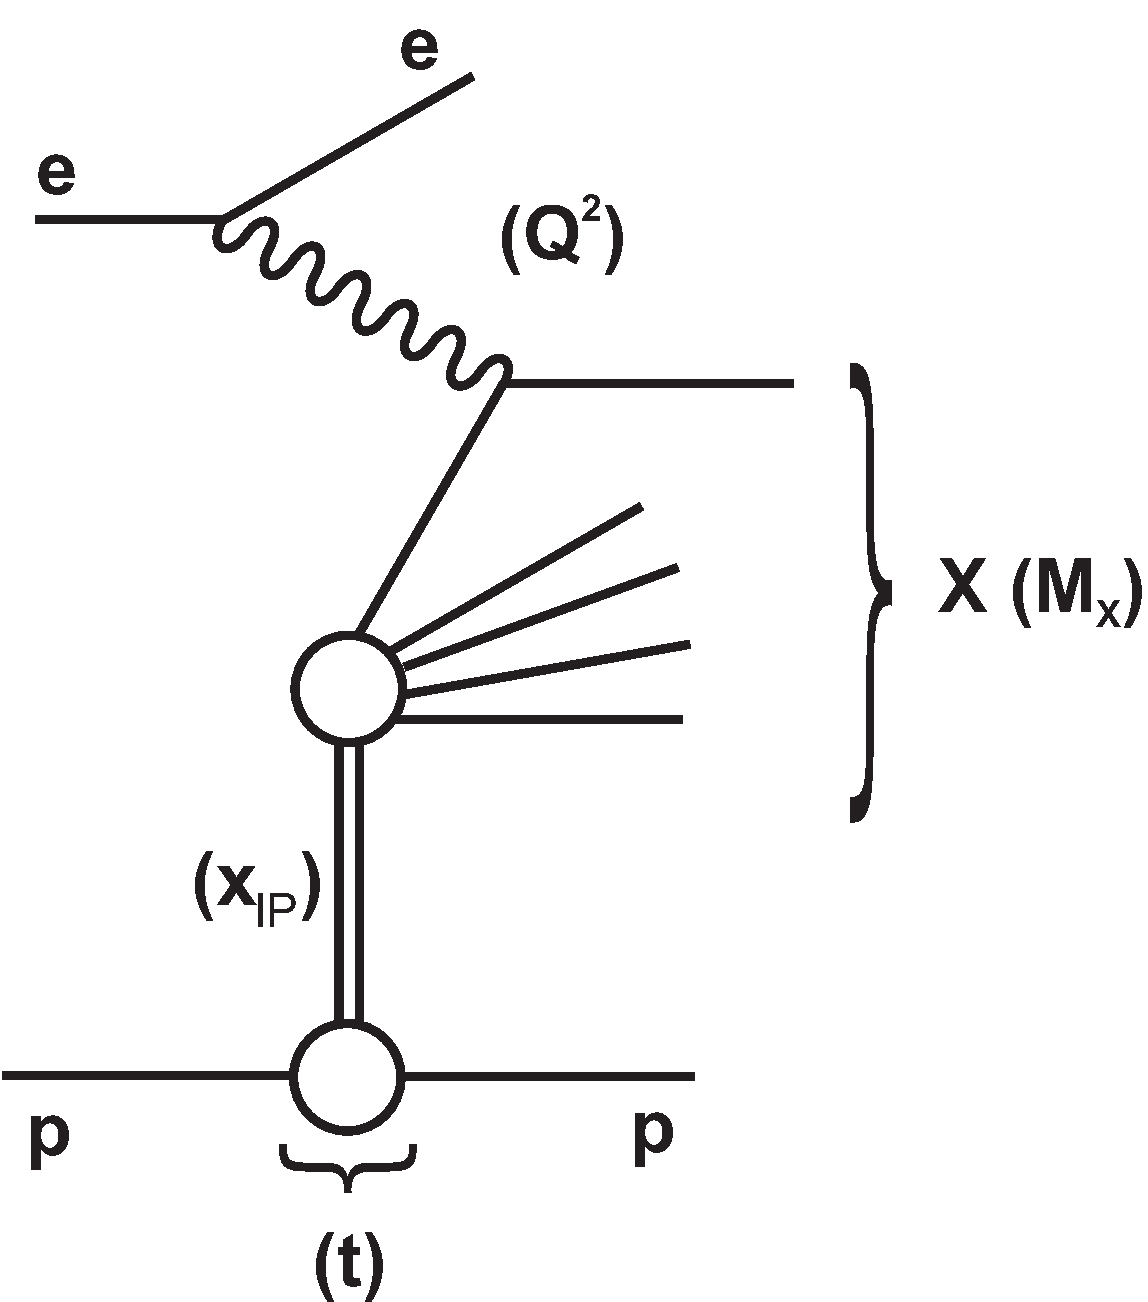
\includegraphics[width=0.5\linewidth]{figures/diffraction.pdf}
%\end{center}
%\caption{Schematic diagram of the kinematic variables used to
% describe the inclusive diffractive DIS process.}
%\label{fig:diff}
%\end{figure}

In addition to the usual variables $x$, $Q^2$, one must consider the squared four-momentum transfer $t$
(the undetected momentum transfer to the proton system) and
the mass $M_X$ of the diffractively produced final state. 
In practice, the variable $M_X$ 
is often replaced by $\beta=\frac{Q^2}{M_X^2+Q^2-t}$.
%
In models based on a factorisable Pomeron, $\beta$ may be viewed as the fraction of the
pomeron longitudinal momentum which is carried by the struck parton, $x=\beta x_{\Pom}$.
%The diffractive parton distribution functions (DPDFs) are interpreted as probabilities for 
%finding a parton with a small fraction of the proton momentum $x=\beta\Pom$

For the inclusive case, the diffractive cross-section can be expressed as:
\begin{equation}
\begin{array}{lcl}
  \frac{d\sigma}{d\beta\,dQ^2dx_{\Pom}\,dt}
=
  \frac{2\pi\alpha^2}{\beta Q^4}\,
    \left( 1 +  (1-y)^2 \right) \ensuremath{\overline\sigma}^{D(4)}(\beta,Q^2,x_{\Pom},t)
\label{Dxs}
\end{array}
\end{equation}
where the ``reduced cross-section'' , $\overline\sigma$, is defined as
\begin{equation}
\begin{array}{lcl}
\overline\sigma^{D(4)}
 = F_2^{D(4)} - \frac{y^2}{1 +  (1-y)^2}\, F_L^{D(4)}
 = F_T^{D(4)} + \frac{2(1-y)}{1 +  (1-y)^2}\, F_L^{D(4)}.
\label{eq:sigred}
\end{array}
\end{equation}
%The dimension of $F_k^{D(4)}(\beta,Q^2,x_{\Pom},t)$
%is $GeV^{-2}$ and thus quantities integrated over $t$.
%\begin{equation}
%F_k^{D(3)}(\beta,Q^2,x_{\Pom})
%\equiv
%\int_{t_{\rm min}}^{t_{\rm max}} dt
%F_k^{D(4)}(\beta,Q^2,x_{\Pom},t)
%\end{equation}
%are dimensionless. The maximum kinematically allowed value of $t$ is given by
%\begin{equation}
%t_{\rm MAX} 
%=
%-\frac{x_{\Pom}^2 m_p^2 + p_\perp^2}{1-x_{\Pom}}
%\approx 
%-\frac{x_{\Pom}^2}{1-x_{\Pom}} m_p^2
%\end{equation}
%where $m_p$ is the proton mass.
With $x = x_{\Pom}\beta$ we can relate this to the standard DIS formula.
%\begin{equation}
%\begin{array}{lcl}
%\frac{d\sigma}{d\beta\,dQ^2\,dx_{\Pom}\,dt} =
%  \frac{2\pi\alpha^2}{x\, Q^4}\,
%    \left( 1 +  (1-y)^2 \right) x_{\Pom}\ensuremath{\overline\sigma}^{D(4)}(\beta,Q^2,x_{\Pom},t)
%\end{array}
%\end{equation}
%which upon integration over $t$ reads
%\begin{equation}
%\begin{array}{lcl}
%\label{Dxs3}
%  \frac{d\sigma}{d\beta\,dQ^2\,dx_{\Pom}}
%=  
%  \frac{2\pi\alpha^2}{x Q^4}\,
%    \left( 1 +  (1-y)^2 \right) \,x_{\Pom}\ensuremath{\overline\sigma}^{D(3)}(\beta,Q^2,x_{\Pom}).
%\end{array}
%\end{equation}
%%The H1 and ZEUS data files typically contain $x_{\Pom}\ensuremath{\overline\sigma}^{D(3)}$.
The diffractive structure functions can be expressed as convolutions of the
calculable coefficient functions with diffractive quark and gluon distribution functions,
 which in general depend on all of \xpom, $Q^2$, $\beta$, $t$.
\\
\\
%==========================================
%{\bf Regge factorization} 
%Needed? \\
The diffractive PDFs in \fitter\ are implemented following the prescription of ZEUS
publication~\cite{zeus:diff2009} and can be used to reproduce the main results.
%For a  better description of data, a contribution from a secondary Reggeon, $\Reg$, is included, hence
%\begin{equation}
%F_k^{D(4)}(\beta,Q^2,x_{\Pom},t) = 
%\sum_{\mathcal{X} =\Pom,\Reg}
%\phi_\mathcal{X}(x_{\Pom},t)\, F^\mathcal{X}_k(\beta,Q^2)
%\end{equation}
%or
%\begin{equation}
%\label{eq:FD3}
%F_k^{D(3)}(\beta,Q^2,x_{\Pom}) = 
%\sum_{\mathcal{X} =\Pom,\Reg}
%\Phi_\mathcal{X}(x_{\Pom})\, F^\mathcal{X}_k(\beta,Q^2)
%\end{equation}
%where
%\begin{equation}
%\label{eq:intFlux}
%\Phi_{\mathcal{X}}(x_{\Pom}) =
%\int\limits_{t_{\rm min}}^{t_{\rm max}} dt\, \phi_\mathcal{X}(x_{\Pom},t)
%\,.
%\end{equation}
%The fluxes are parametrized as
%\begin{subequations}
%\label{eq:flux}
%\begin{equation}
%\phi_\mathcal{X}(x_{\Pom},t) = 
%\frac {A_\mathcal{X}\, e^{b_\mathcal{X} t}} {x_{\Pom}^{2\alpha_\mathcal{X}(t) -1}}
%\end{equation}
%where
%\begin{equation}
%\alpha_\mathcal{X}(t) = \alpha_\mathcal{X}(0) + \alpha_\mathcal{X}' t
%\,.
%\end{equation}
%\end{subequations}
%The function $F^\Reg_k(\beta,Q^2)$  is taken to be that of the pion.
%